% !TeX encoding = utf8
% !TeX spellcheck = en_US

\section{Results}
\begin{table*}[ht]
	\centering
	\begin{tabular}{|l|c|c|c|c|c|c|c|}
		\hline
		\multirow{2}{*}{\textbf{Patient 563}} & \multicolumn{1}{c|}{\textbf{Mean $\pm$ Std}} & \multicolumn{6}{c|}{\textbf{Time in range [\%]}} \\ \cline{3-8}
		&  & \textbf{(70-180)} & \textbf{(70-140)} & \textbf{(<70)} & \textbf{(<54)} & \textbf{(>180)} & \textbf{(>250)} \\ \hline
		True                 & 153.4 $\pm$ 55.1    & 0.7    & 0.4    & 0.0    & 0.0    & 0.3    & 0.0    \\ \hline
		Subsampling rate 1   & 153.4 $\pm$ 55.1    & 0.7    & 0.4    & 0.0    & 0.0    & 0.3    & 0.0    \\ \hline
		Subsampling rate 2   & 153.4 $\pm$ 55.0    & 0.7    & 0.4    & 0.0    & 0.0    & 0.3    & 0.0    \\ \hline
		Subsampling rate 4   & 153.3 $\pm$ 55.1    & 0.7    & 0.4    & 0.0    & 0.0    & 0.3    & 0.0    \\ \hline
		Subsampling rate 8   & 153.8 $\pm$ 55.2    & 0.7    & 0.4    & 0.0    & 0.0    & 0.3    & 0.0    \\ \hline
		Subsampling rate 16  & 153.0 $\pm$ 56.1    & 0.7    & 0.4    & 0.0    & 0.0    & 0.3    & 0.0    \\ \hline
		Subsampling rate 32  & 152.3 $\pm$ 50.6    & 0.8    & 0.4    & 0.0    & 0.0    & 0.2    & 0.0    \\ \hline
	\end{tabular}
	\caption{Summary of the performance metrics for Patient 563 across different subsampling rates.}
	\label{tab:patient563}
\end{table*}


\begin{figure*}[ht] % "ht" means "here" or "top", a positioning option
	\centering
	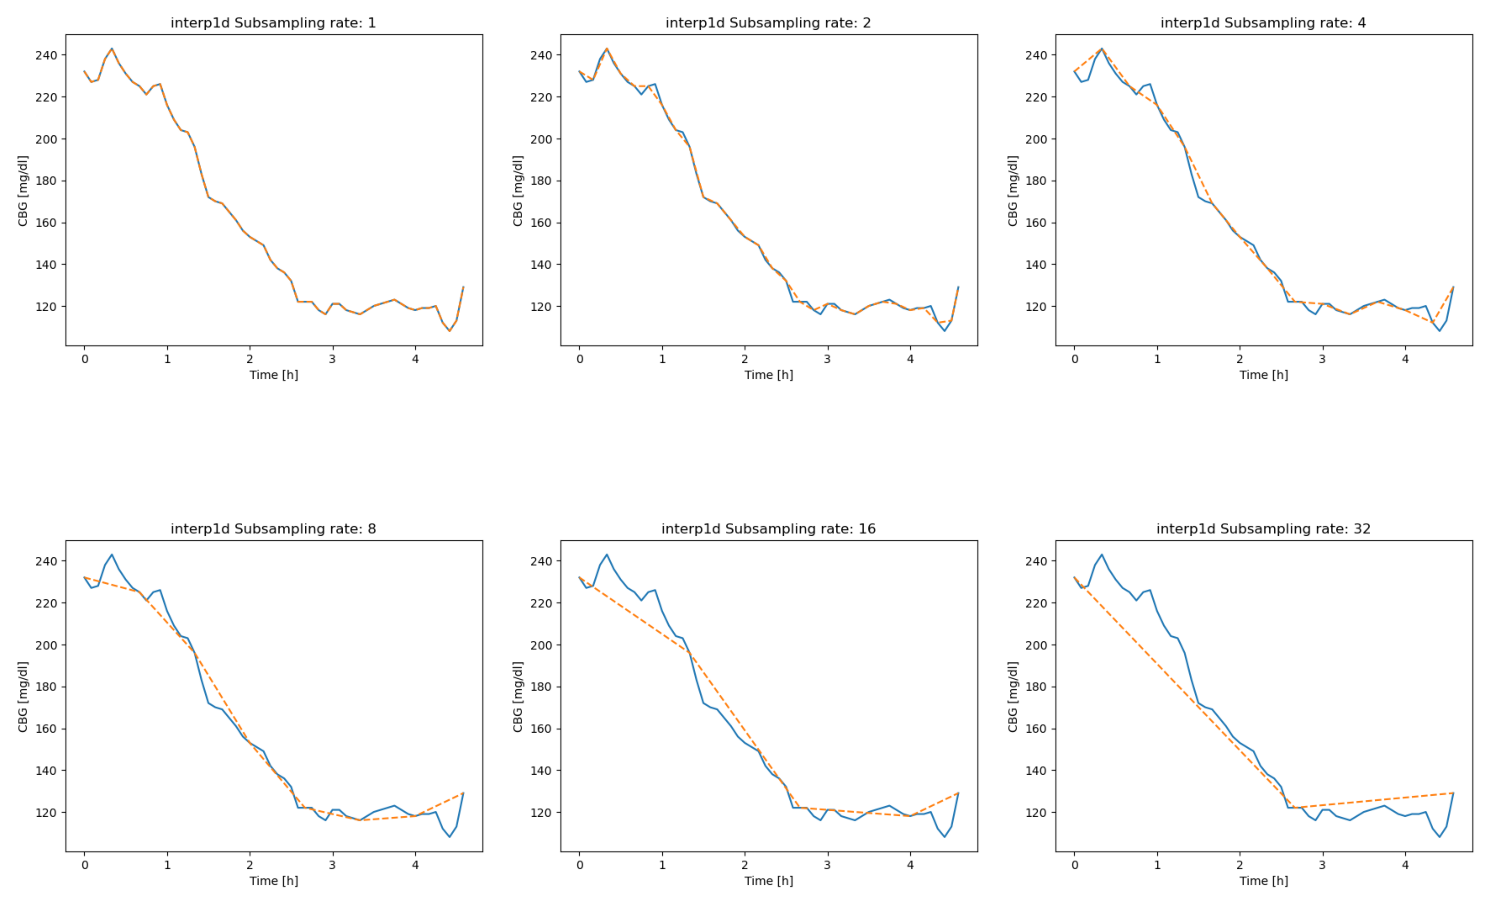
\includegraphics[width=\textwidth]{Figures/SR_combined.png} % Adjust the width as needed
	\caption{Subsampling reconstruction of the true signal for different subsampling rates. The figure shows a 2x3 grid of subplots where each plot represents the reconstructed signal from the true signal using various subsampling rates. The subsampling rates are 1, 2, 4, 8, 16, and 32, respectively, and are visualized to assess the impact of different levels of data reduction on signal fidelity.}
	\label{fig:SR_combined}  % For referencing the figure in the text
\end{figure*}

As shown in Figure \ref{fig:SR_combined}, this is a description of what the figure illustrates.


\begin{figure}[ht] % "ht" means "here" or "top", a positioning option
	\centering
	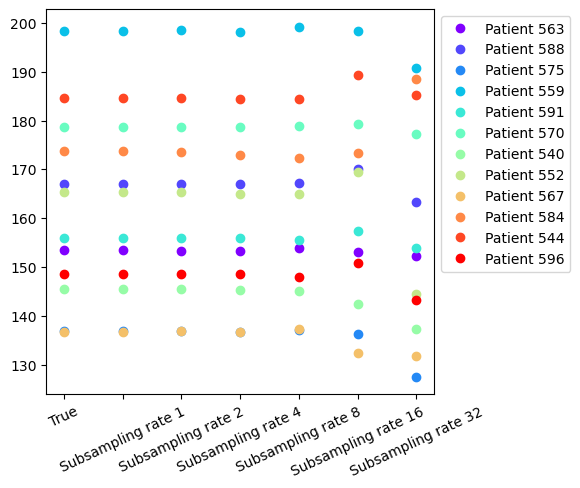
\includegraphics[width=\linewidth]{Figures/patients_mean.png} % Adjust the width as needed
	\caption{Mean blood glucose values across all patients in the dataset for various subsampling rates. The figure illustrates how the mean blood glucose value changes as the subsampling rate increases, highlighting the effect of reduced data resolution on the accuracy of the computed mean. Subsampling rates include 1 (original resolution), 2, 4, 8, 16, and 32, where higher rates correspond to greater data reduction.}
	\label{fig:patients_mean}  % For referencing the figure in the text
\end{figure}

As shown in Figure \ref{fig:patients_mean}, this is a description of what the figure illustrates.

